\documentclass{report}

\usepackage{graphicx}
\usepackage{float}

\begin{document}

\begin{titlepage}
\begin{center}
\large{\bfseries Project proposal}\\
\large{CMPSCI 670, Fall 2019, UMass Amherst}
\end{center}
\textbf{Project title:} Sudoku Solver\\
\newline
\textbf{Team members:} Zhiyi Lai\\
\newline
\textbf{Abstract:}\\

Sudoku is a popular brain game for a long time. While for humans, the game requires some thought, for a computer, it can instantly complete a sudoku game using algorithms.
For this task, I will combined traditional image processing methods to capture Sudoku board image and seperate the image to 81 digits patches, then I will use Convolutional Neural Network to get Sudoku board matrix from the patches.
Finally I will use simple backtracking algorithms to solve the sudoku puzzle and display the result on the video stream.

The whole process is shown in Figure \ref{fig:process}.

\begin{figure}[H]
    \centering
    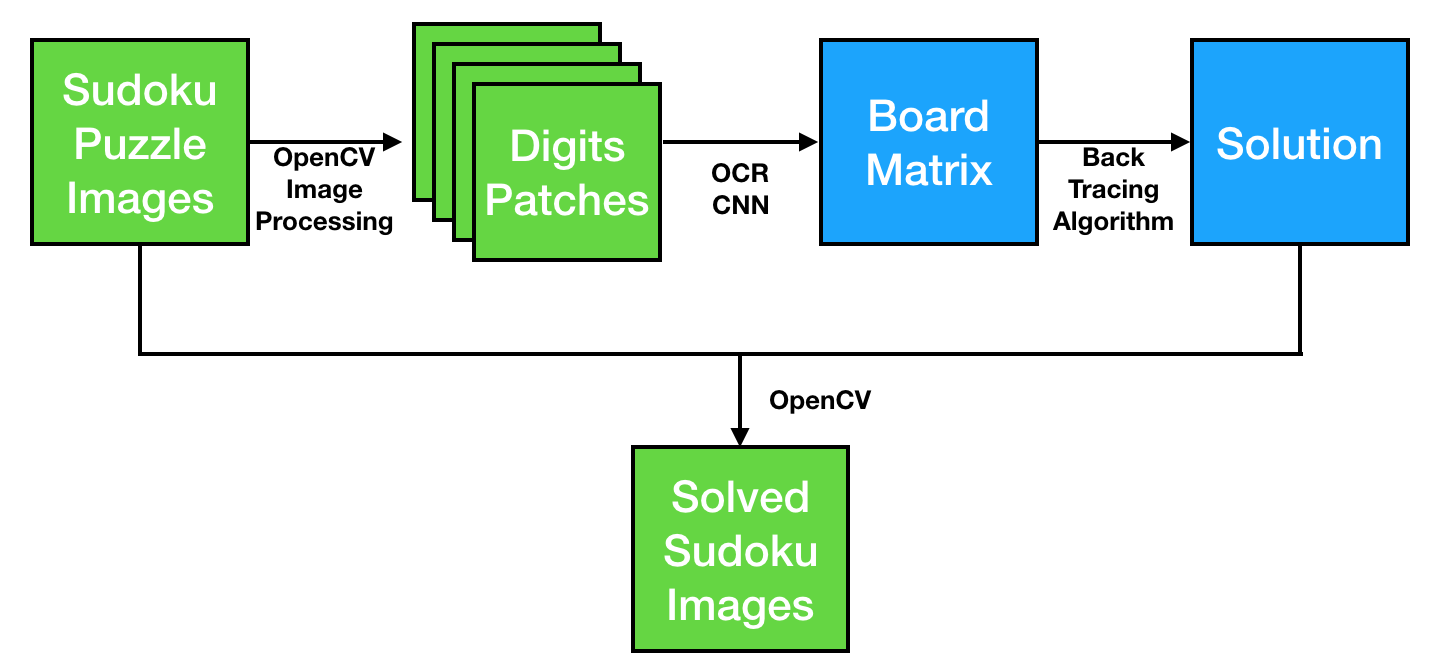
\includegraphics[scale=0.4]{processing.png}
    \caption{Solving Process}
    \label{fig:process}
\end{figure}

In this project, I will use simple labeled sudoku images dataset online for board detection and Chars74K dataset to train the digits recognition model.

\end{titlepage}

\end{document}